\begin{figure}[!hbt]
\centering
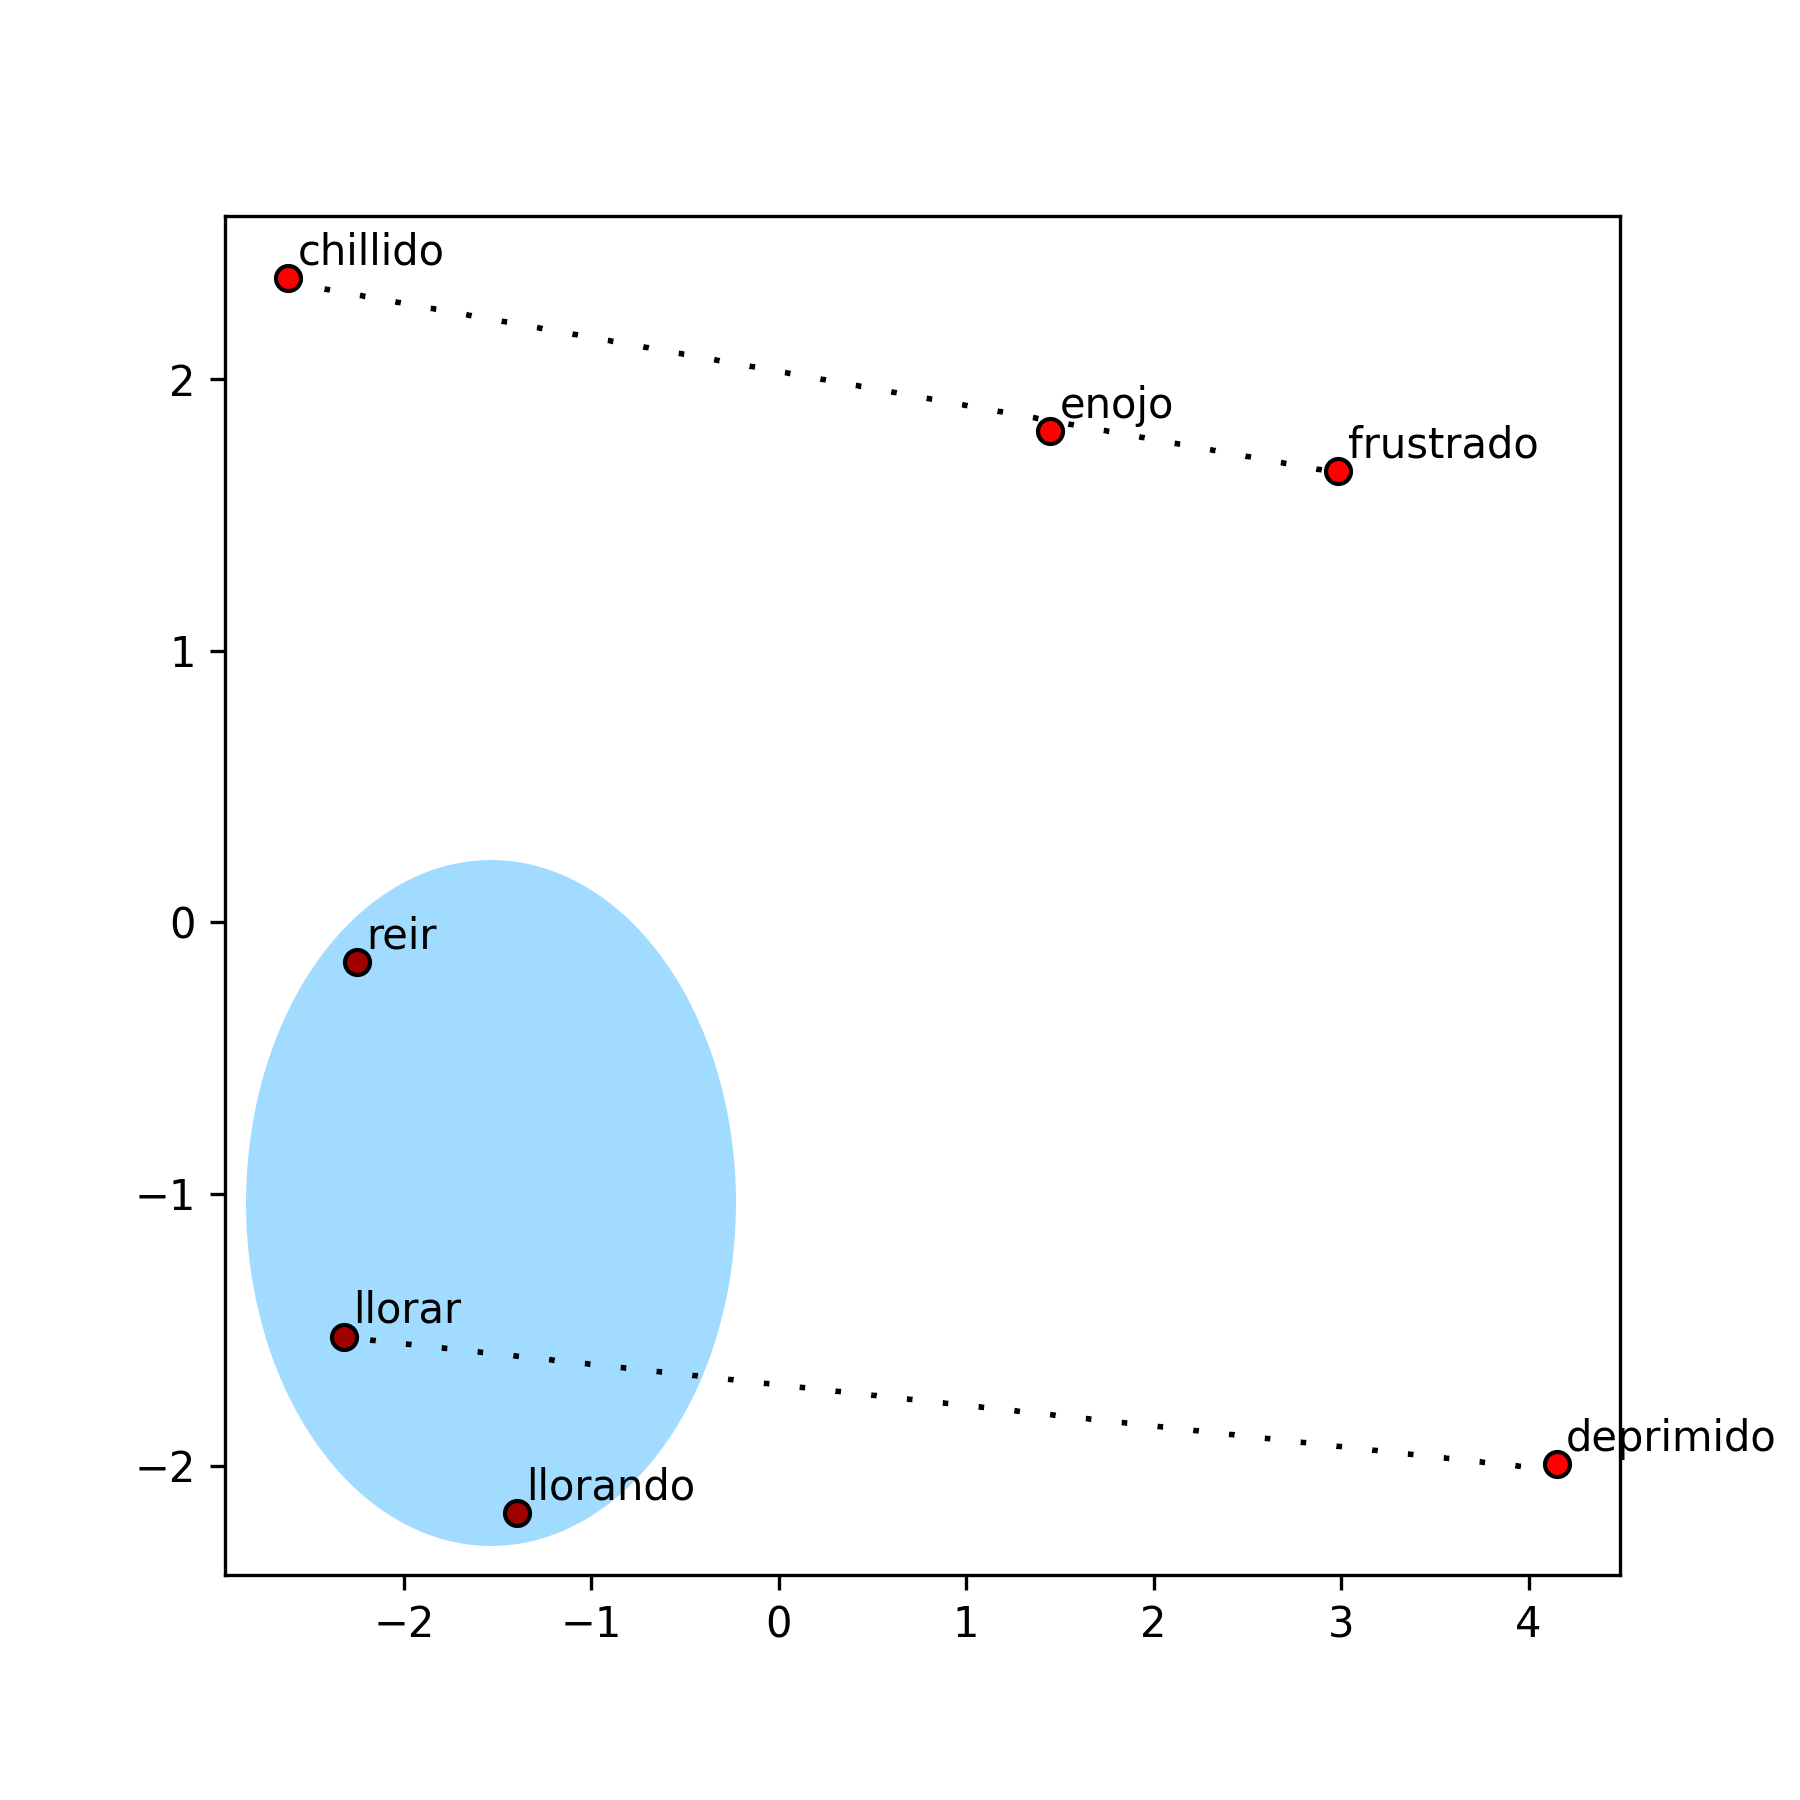
\includegraphics[width=0.7 \textwidth]{sections/figures/analogia.png}
\caption{Palabras que ocurren en contextos de uso similares tienen una similitud relacional alta, incluyendo el caso de antónimos, por ejemplo \textit{llorar} vs \textit{reír} }
\label{fig:analogia}
\end{figure}